% --
% dataset

\section{Dataset}\label{sec:exp_dataset}
\thesisStateReady
Two datasets are used within this thesis, one is the second version of the speech commands dataset \cite{Warden2018} and the other is self made consisting of only 5 labels (speech commands) that are especially valuable for movement in video games.
The self made dataset is denoted as \enquote{my dataset} and it is merely used for evaluation.
The training, validation and testing of the neural network architectures is performed on the speech commands dataset.
Both datasets consists of raw waveform files in the \texttt{.wav} format without any feature extraction done beforehand.
As already mentioned in \rsec{prev_kws_benchmark}, the direct comparisons between different neural network approaches is difficult if the feature extraction is left alone to the user.
Some datasets provide feature extraction beforehand, so that the comparability of neural network architectures performances is not influenced on it.
The speech commands dataset does not explicitly separate each \texttt{.wav} file into train, test and validation sets, but provides file lists that refers to distinct waveform files that should be used for testing and validation and therefore provides means for comparison to researchers.
More details about the datasets is presented below.

% Some abbreviations and references were done, so that the jungle of selected parameters get a little bit more clear to the reader of this thesis.in the \texttt{.wav} format
% The abbreviations of the dataset are shown in \rtab{exp_dataset_abbr}.

% The speech commands dataset is extracted before it is used for training. 
% To reduce computations in the evaluation process of neural networks, it was important to reduce the number of classes and examples per class to an suitable number.

% \begin{table}[ht!]
\begin{center}
\caption{Dataset abbreviations for label selection and feature group extraction.}
\begin{tabular}{ M{2cm} M{9cm} }
\toprule
%\multicolumn{4}{c}{\textbf{Feature Groups}} & \multicolumn{2}{c}{\textbf{Accuracy}} \\
\textbf{Abbreviation} & \textbf{Meaning}\\
\midrule
L5 & Selected labels: left, right, up, down, go\\
L10 & Selected labels: yes, no, left, go, down, off, right, stop, up, on\\
L30 & Selected labels: \enquote{all}\\
n[0-9]+ & Number of examples per class label, e.g. n500\\
\midrule
c[0-1] & Feature Group, use of cepstral features, 0 is false and 1 is true\\ 
d[0-1] & Feature Group, use of delta features, \ditto\\ 
dd[0-1] & Feature Group, use of double delta features, \ditto\\ 
e[0-1] & Feature Group, use of energy features, \ditto\\
norm[0-1] & features are normalized over frames\\
\bottomrule
\label{tab:exp_dataset_abbr}
\end{tabular}
\end{center}
\vspace{-4mm}
\end{table}
\FloatBarrier
\noindent



% --
% speech commands dataset

\subsection{Speech Commands Dataset}\label{sec:exp_dataset_speech_cmd}
The speech command dataset \cite{Warden2018} exists in two versions (\texttt{v0.01} and \texttt{v0.02}).
The first version was published in 2017 and the second emerged as improved version of the first with 5 more key words \{\enquote{backward}, \enquote{forward}, \enquote{follow}, \enquote{learn}, \enquote{visual}\}, class examples and better quality check in 2018.
The dataset consists of \SI{1}{\second} speech recordings of 30 different words in \texttt{v0.01} and 35 different words in \texttt{v0.02}, done by over thousands of individual speakers.

In this thesis, the experiments are done on the second version \texttt{v0.02} of the dataset with hard-facts listed in \rtab{exp_dataset_hard_facts}.
% hard facts
\begin{table}[ht!]
\begin{center}
\caption{Hard facts of the speech commands dataset \texttt{v0.02}.}
\begin{tabular}{ M{5cm}  M{2cm} }
\toprule
%\textbf{label} & \textbf{train} \\
%\midrule
Total number of key words & 35\\
Total number of examples & 105886\\
Total number of speakers & 2618\\
\midrule
%Number of core key words & 20\\
%Number of auxiliary key words & 15\\
Recording duration & 0.4 - \SI{1}{\second}\\
Channels & Mono\\
Bit depth of audio files & \SI{32}{\bit}\\
Sampling frequency & \SI{16}{\kilo\hertz}\\
\bottomrule
\label{tab:exp_dataset_hard_facts}
\end{tabular}
\end{center}
\end{table}
\FloatBarrier
\noindent


All speech command key words with their separation in training, test and validation set are shown in \rtab{exp_dataset_all_labels} loacated in the appendix.
% all labels tab
%\begin{table}[ht!]
\small
\begin{center}
\caption{All labels and counts of available data examples for each set, obtained from the speech commands dataset \texttt{v0.02}.}
\begin{tabular}{ M{2cm}  M{1.75cm}  M{1.75cm}  M{1.75cm}  M{1.75cm} }
\toprule
\textbf{label} & \textbf{train} & \textbf{test} & \textbf{validation} & \textbf{total} \\
\midrule
backward & 1346 & 165 & 153 & 1664 \\
bed & 1624 & 234 & 213 & 2071 \\
bird & 1697 & 185 & 182 & 2064 \\
cat & 1657 & 194 & 180 & 2031 \\
dog & 1711 & 220 & 197 & 2128 \\
down & 3134 & 406 & 377 & 3917 \\
eight & 3033 & 408 & 346 & 3787 \\
five & 3240 & 445 & 367 & 4052 \\
follow & 1275 & 172 & 132 & 1579 \\
forward & 1256 & 155 & 146 & 1557 \\
four & 2955 & 400 & 373 & 3728 \\
go & 3106 & 402 & 372 & 3880 \\
happy & 1632 & 203 & 219 & 2054 \\
house & 1727 & 191 & 195 & 2113 \\
learn & 1286 & 161 & 128 & 1575 \\
left & 3037 & 412 & 352 & 3801 \\
marvin & 1710 & 195 & 195 & 2100 \\
nine & 3170 & 408 & 356 & 3934 \\
no & 3130 & 405 & 406 & 3941 \\
off & 2970 & 402 & 373 & 3745 \\
on & 3086 & 396 & 363 & 3845 \\
one & 3140 & 399 & 351 & 3890 \\
right & 3019 & 396 & 363 & 3778 \\
seven & 3205 & 406 & 387 & 3998 \\
sheila & 1606 & 212 & 204 & 2022 \\
six & 3088 & 394 & 378 & 3860 \\
stop & 3111 & 411 & 350 & 3872 \\
three & 2966 & 405 & 356 & 3727 \\
tree & 1407 & 193 & 159 & 1759 \\
two & 3111 & 424 & 345 & 3880 \\
up & 2948 & 425 & 350 & 3723 \\
visual & 1288 & 165 & 139 & 1592 \\
wow & 1724 & 206 & 193 & 2123 \\
yes & 3228 & 419 & 397 & 4044 \\
zero & 3250 & 418 & 384 & 4052 \\
\_noise\footnotemark & 2863 & 357 & 357 & 3577 \\
\bottomrule
\label{tab:exp_dataset_all_labels}
\end{tabular}
\end{center}
\vspace{-4mm}
\end{table}
\FloatBarrier
\noindent
\footnotetext{The noise label was added from the provided noise files, as described in \rsec{exp_dataset_structure}.}
Some labels have a significantly higher number of example than others do.
%In \rtab{exp_dataset_all_labels} it can be observed, that some labels are occurring significantly more often than others.
The inconsistent number of the total number of examples per label, emerged from the recording settings as described in \cite{Warden2018}, where the more important words were recorded with a higher number of iterations from the same speaker, for instance the speaker has to create five samples of \enquote{go} and two of \enquote{marvin}.
This makes the key words separable into into \emph{core key words} and \emph{auxiliary key words}.
The core key words are the main classification objective and each core key word should corresponds to one class label, therefore the core key words have the higher count of samples with about 3000 to 4000 examples each.
In detail the core key words are \{\enquote{yes}, \enquote{no}, \enquote{up}, \enquote{down}, \enquote{left}, \enquote{right}, \enquote{on}, \enquote{off}, \enquote{stop}, \enquote{go}, \enquote{zero}, \enquote{one}, ..., \enquote{nine} \}.

The auxiliary key words have the purpose to disturb the classification of the core key words, therefore the auxiliary key words should be represented by a single class label.
In many papers those auxiliary key words are labeled with \enquote{unknown}, but in this thesis it is referred as \enquote{\_mixed} label, since it is a mixture of all auxiliary key words and the core words that were not used for classification.
The \enquote{\_mixed} key words should represent all unknown words that a user might speak and are therefore a very important element in the KWS task for the identification of words that are not in the class dictionary.
Note that the \enquote{\_mixed} label makes the classification task much more challenging, because the network has to be more accurate in modeling the core key words against the other key words.
In the creation of the examples for the \enquote{\_mixed} label, it is of course preferable to have equal amounts of examples per individual auxiliary key word and unused core key words.
This had been done by placing all unused core key words and auxiliary words into a separate folder and reading them into a list, which is ordered so that one example per key word is placed consecutive to the next for each key word, then it starts over again filling up all examples.
The number of examples picked for training is then simply the entries from index 0 to the number of examples in training. 

To examine the recorded examples, one example per label from the speech command dataset in raw audio format is shown in \rfig{exp_dataset_speech_cmd_wav_grid}.
\begin{figure}[!ht]
  \centering
    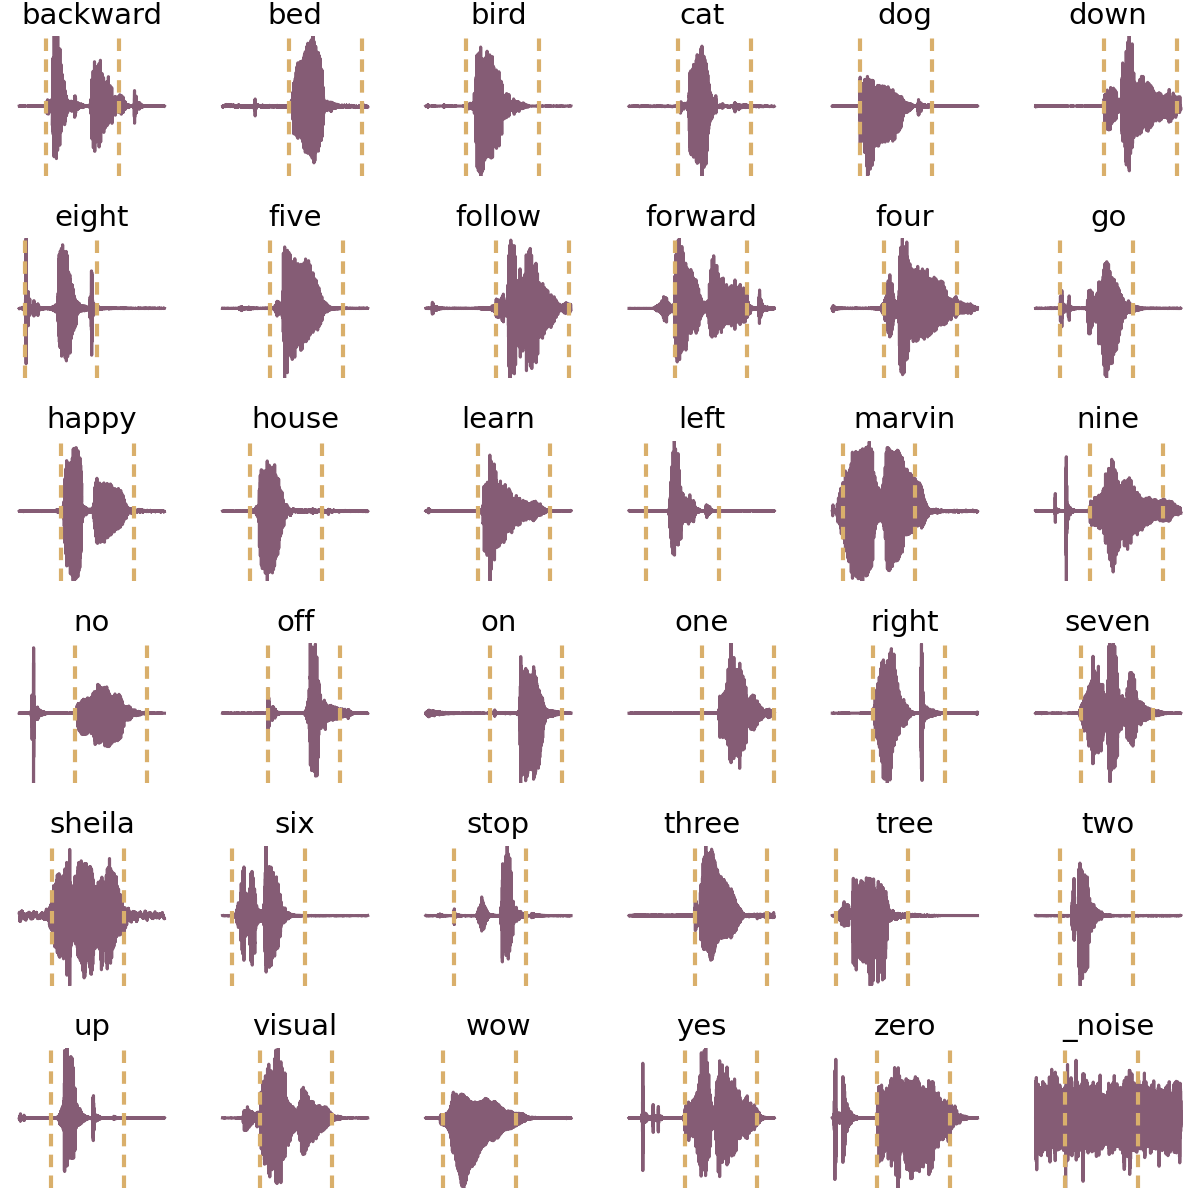
\includegraphics[width=0.65\textwidth]{./5_exp/figs/exp_dataset_speech_cmd_wav_grid}
  \caption{One random sample of each individual speech command in the speech command dataset in normalized raw audio format.}
  \label{fig:exp_dataset_speech_cmd_wav_grid}
\end{figure}
\FloatBarrier
\noindent


% --
% statistics

\subsubsection{Observations of all examples in the dataset}
Two histograms were created to observe the quality of all recorded files, those are an energy measure for each file and the count of the sample length.
The energy of a recorded file provides information about a recordings amplification setting and is an indicator for too silent or too loud (overdrive distortions) samples. 
In the first version of the speech command dataset (\texttt{v0.01}) too silent files were a problem, this had been fixed in the second version by rejecting those silent files, therefore \texttt{v0.01} is a bit more unclean than \texttt{v0.02}.
The energy value $e \in \R$ can be computed as:
\begin{equation}\label{eq:exp_dataset_energy}
  e = \frac{1}{n} \left( x^T\, x \right)
\end{equation}
where $x \in \R^n$ are the values of all samples from the recorded files.
The division through the length of each individual audio recording of a total number of samples $n$, has to be done, because not every file has a duration of \SI{1}{\second} corresponding to 16000 samples.
For an unknown reason some of the recordings have less than 16000 samples.
It would be problematic if the sample length is too low to capture a word, but the minimum duration of all files is about \SI{0.4}{\second}, and this is enough for words like \enquote{go}.
The histograms of all available examples in the dataset are shown in \rfig{exp_dataset_hist}.

\begin{figure}[!ht]
  \centering
    \subfigure[energy]{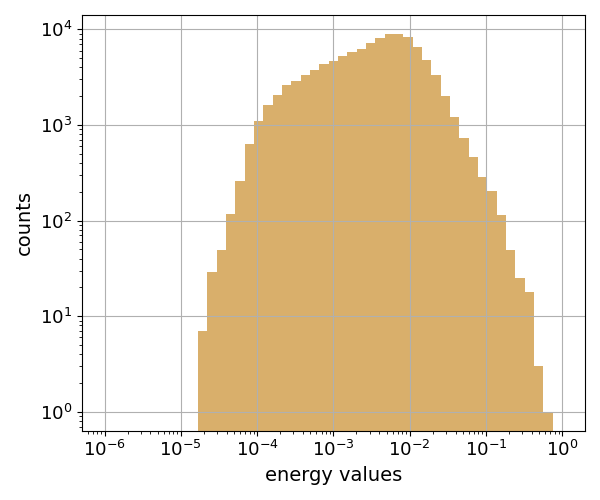
\includegraphics[width=0.45\textwidth]{./5_exp/figs/exp_dataset_hist_energy_overall}}
    \subfigure[sample length]{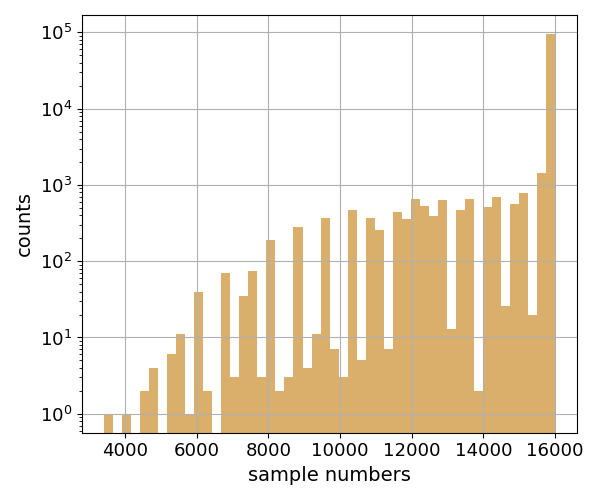
\includegraphics[width=0.45\textwidth]{./5_exp/figs/exp_dataset_hist_sample_overall}}
  \caption{Energy value and sample length histograms in log-log and log-scale respectively of all examples in the speech commands dataset \texttt{v0.02}.}
  \label{fig:exp_dataset_hist}
\end{figure}
\FloatBarrier
\noindent
The energy histogram has one main lobe, which is good, so it means that there are no clusters of extremely silent or loud files.
For comparison, if silent files were extracted from for instance the given background files, the energy of some of those is in range of $10^{-7} \dots 10^{-6}$. Therefore it seems that most of the files are okay.
The sample length histogram shows, that most of the files have a duration of \SI{1}{\second}, but many other have less sample numbers. 
This is important and has to be regarded in the pre-processing of audio files, because inputs to neural networks must often be prepared to fixed size inputs if no sequential neural networks are deployed, such as Recurrent Neural Networks (RNN).


% --
% recording quality

\subsubsection{Recording Quality and Personal Experience}
The examples of the speech commands dataset \cite{Warden2018} were not recorded by professionals with high-end recording equipment, in fact the recordings had been done in an amateur kind of fashion, so that the dataset is more suited to realistic environments intended for user applications.
This is also noted in the paper \cite{Warden2018}:
\begin{quote}
...This meant that the use of studio-captured samples seemed unrealistic, since that audio would lack background noise, would be captured with high-quality microphones, and in a formal setting. 
Successful models would need to cope with noisy environments, poor quality recording equipment, and people talking in a natural, chatty way...
\end{quote}
The recording devices of the speakers, who contributed examples to the dataset, were in most cases simple consumer microphones, as for instance deployed in laptops or mobile phones.

The personal experiments made, when listening to the examples in the dataset, were as follows:
\begin{itemize}
  \item The quality of the examples in the dataset are ranging from really good and understandable to very bad, noisy, unrecognizable and cut off, though most of the examples are good.

  \item Different accents had been perceived, that suggests that people from several nationalities were involved. 
  However the bias was laid on American English, as noted in the paper.

  \item No children speakers had been found in the personal listening of examples.
\end{itemize}

Due to data privacy issues the information of individual speakers is not displayed.
Further it is not clear if there are equal amounts of male and female speakers and if there are any children speakers included.
The last would be especially interesting for a video games suited for kids.

In many recordings the background noise is imminent, such as traffic noise, chattering people, office sounds, etc.
A quality check of the recorded files in the dataset had been done beforehand, to ensure that bad samples were rejected.
However there are still some existing flaws such as extremely loud or silent recordings, examples with inconsistent sample numbers, recordings that are including too much noise or in the worst case, noise only (very rarely) and cut off samples where only half of a word had been captured.
Those quality issues in the dataset can for most cases be neglected or fixed, such as inconsistent sample numbers. 
Other more problematic cases, for instance noise-only examples, should actually be filtered out, but since their occurrence is very rare, it is not worth the effort.
Usually it is not a problem for neural networks to cope with noisy datasets. 
Actually it is favorable if the dataset contains many noisy samples, so that neural networks can learn invariances against noise, loudness differences and other nuisances during training.
Further if the training dataset is large enough and the test and validation sets do not contain very bad examples, there should be no problem in the training and evaluation of different models.
Finally it has to be acknowledged that the dataset is under the creative common license freely available to everyone, which is simply fabulous.


% --
% dataset structure

\subsubsection{Dataset Structure}
The speech command examples are stored in separate folders named after each individual key word, in the \texttt{.wav} format.
The folder named as \texttt{\_background\_noise\_} contains six different background noise files, such as \texttt{white\_noise.wav} or \texttt{doing\_the\_dishes.wav}, with a duration of more than one minute each.
Noise examples with a new noise label named \texttt{\_noise} were extracted from those background noise files with a \SI{1}{\second} window shifted by \SI{0.2}{\second}.

Each waveform file is named with an 8-digit hexadecimal hash code for the speaker identification, followed by the utterance number, for instance \texttt{3b4f8f24\_nohash\_0.wav}.
Therefore it is possible to distinguish between different speakers, however as mentioned above, no further information about the speaker is given due to data privacy issues.

Further the dataset provides a testing file list called \texttt{testing\_list.txt} and a validation file list \texttt{validation\_list.txt} where each row entry refers to a file in the dataset, for example \texttt{right/bb05582b\_nohash\_3.wav}.
Those file lists for testing and validation should ensure the comparability between different neural network approaches from individual researchers.
The testing and validation file lists are applied in this thesis and the separation into sets are shown in \rtab{exp_dataset_all_labels}.

% --
% extracted examples

\subsubsection{Samples from the Feature Extraction}
The feature extraction of the dataset with specified parameters and storage of the extracted features and labels as separate files is done beforehand, so that it does not have to be applied each time a training instance of a neural network is performed.
Samples from the Mel Frequency Cepstral Coefficients (MFCC) with frame based normalization as explained in \rsec{signal_mfcc} are shown in \rfig{exp_dataset_speech_cmd_mfcc}.
\begin{figure}[!ht]
  \centering
    \subfigure[left]{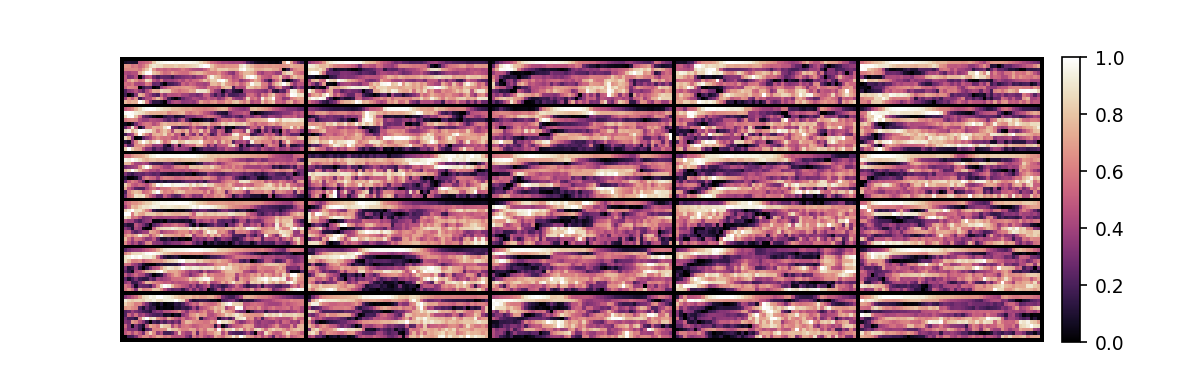
\includegraphics[width=0.45\textwidth]{./5_exp/figs/exp_dataset_speech_cmd_mfcc_left}}
    \subfigure[right]{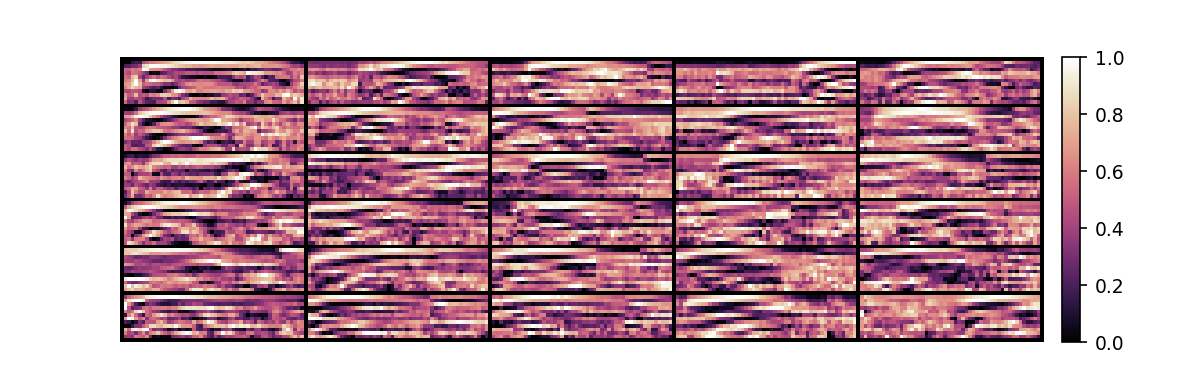
\includegraphics[width=0.45\textwidth]{./5_exp/figs/exp_dataset_speech_cmd_mfcc_right}}
    \subfigure[up]{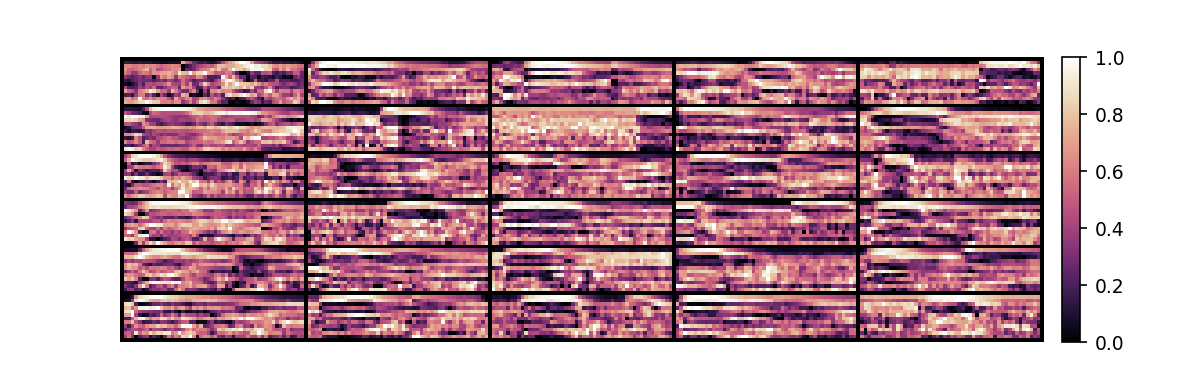
\includegraphics[width=0.45\textwidth]{./5_exp/figs/exp_dataset_speech_cmd_mfcc_up}}
    \subfigure[down]{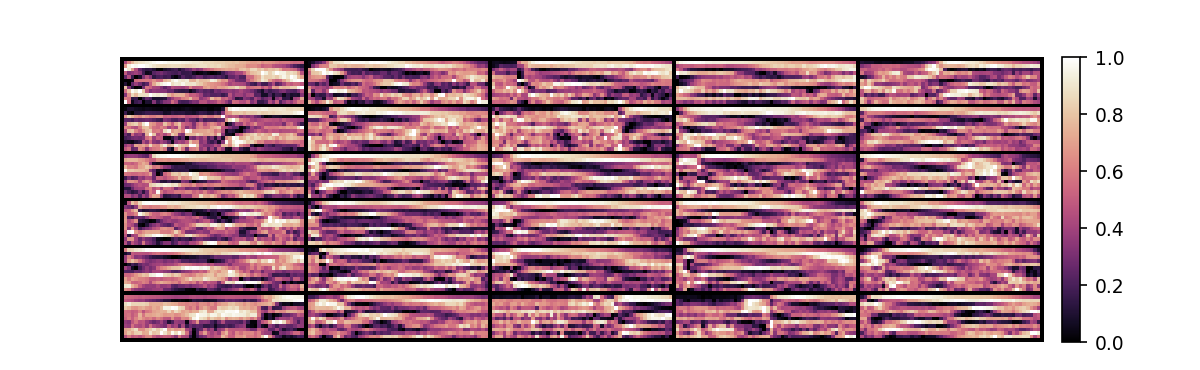
\includegraphics[width=0.45\textwidth]{./5_exp/figs/exp_dataset_speech_cmd_mfcc_down}}
    \subfigure[go]{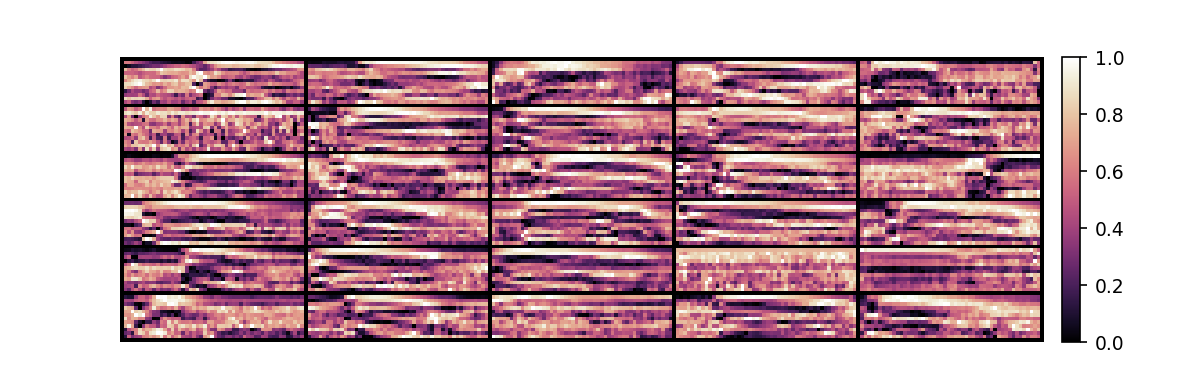
\includegraphics[width=0.45\textwidth]{./5_exp/figs/exp_dataset_speech_cmd_mfcc_go}}
  %\caption{MFCC extracted samples of specific labels obtained from the training set of the speech commands dataset \texttt{v0.02}.}
  \caption{MFCC extraction of randomly selected 30 samples per class label, obtained from the training set of the speech commands dataset \texttt{v0.02}. The corresponding class labels are written below the plots.}
  \label{fig:exp_dataset_speech_cmd_mfcc}
\end{figure}
\FloatBarrier
\noindent


% --
% my dataset

\subsection{My own Dataset}\label{sec:exp_dataset_my}
This dataset was created by the author of this thesis and contains five examples for each of the following key words \{\enquote{left}, \enquote{right}, \enquote{up}, \enquote{down} and \enquote{go}\}.
The datasets purpose is mainly to have an additional test set for evaluating trained models on the authors own voice.
The examples per key word are spoken with different emphasis and stress on individual phonemes for each key word.
Also the prolongation of the words are different, for instance that in one example the word is spoken very hasty and in the other it is spoken slowly.
The emphasis and prolongation ensure the diversity of the dataset. 
It is important to mention that none of the self recorded files were used within the training set, so that the neural networks performance is evaluated on unseen data.
All examples of my own dataset are illustrated in \rfig{exp_dataset_my_wav_grid} in raw audio format.
\begin{figure}[!ht]
  \centering
    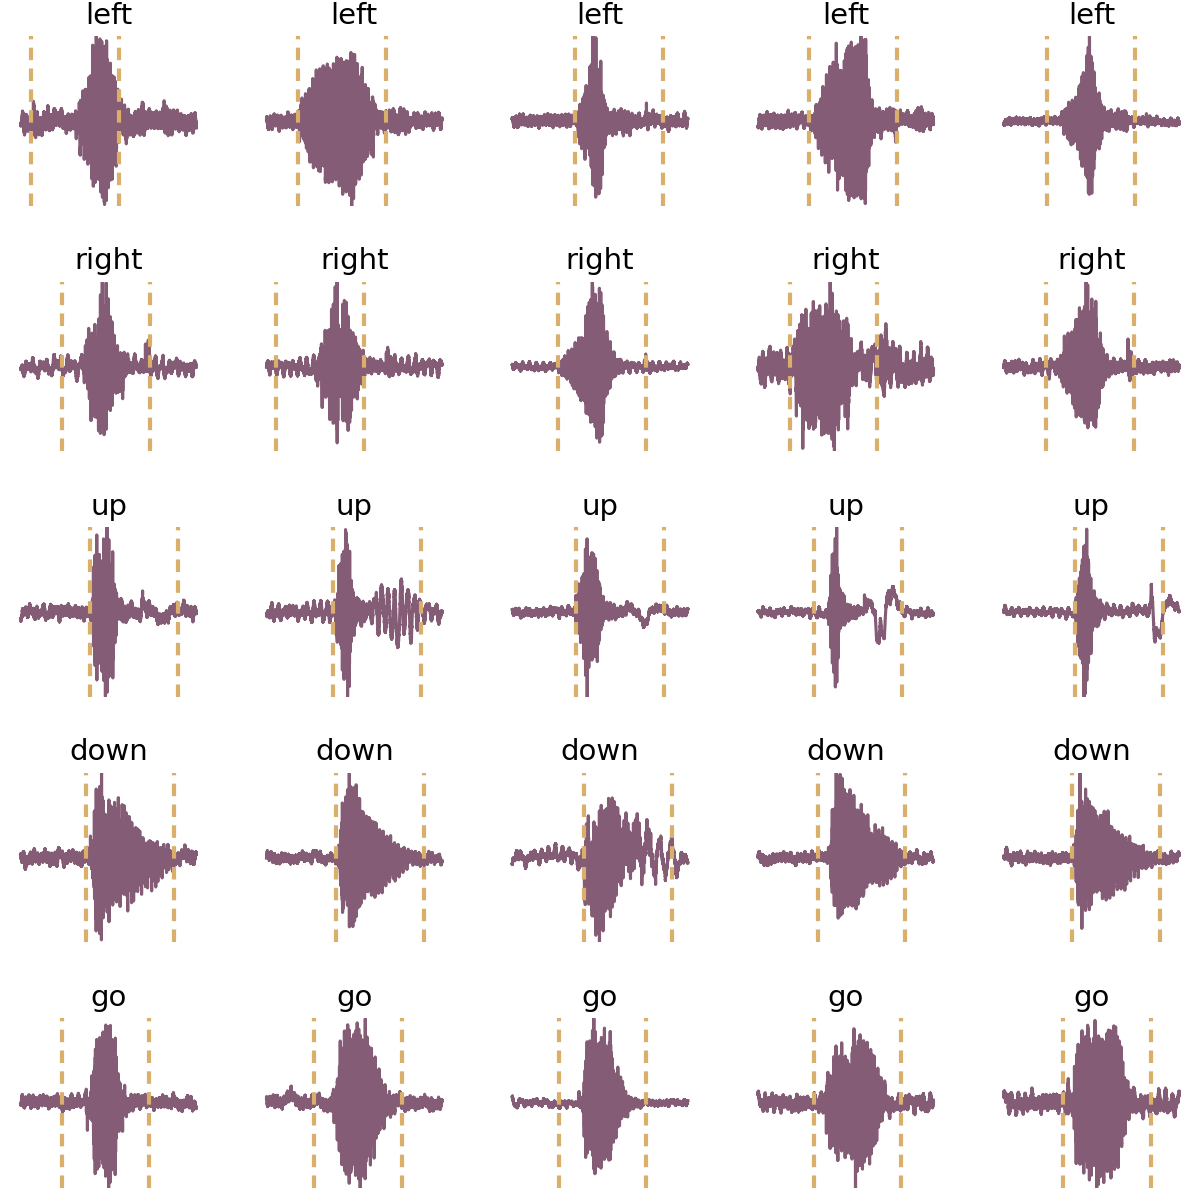
\includegraphics[width=0.65\textwidth]{./5_exp/figs/exp_dataset_my_wav_grid}
  \caption{Self recorded files of the \enquote{my dataset} in raw audio format.}
  \label{fig:exp_dataset_my_wav_grid}
\end{figure}
\FloatBarrier
\noindent
The same examples extracted to MFCC features are shown in \rfig{exp_dataset_my_mfcc}.
\begin{figure}[!ht]
  \centering
    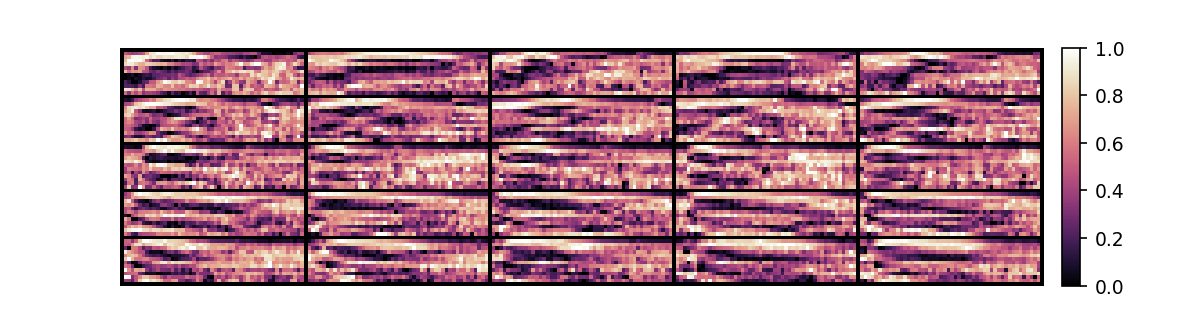
\includegraphics[width=0.65\textwidth]{./5_exp/figs/exp_dataset_my_mfcc}
  \caption{All MFCC extracted samples of the \enquote{my dataset} with the same ordering as shown in \rfig{exp_dataset_my_wav_grid}.}
  \label{fig:exp_dataset_my_mfcc}
\end{figure}
\FloatBarrier
\noindent
It turned out that it is a very hard task for neural networks to achieve a $100\%$ classification score upon it, even though all examples are from the same speaker.
This is a bit worrying, because acoustically each of the examples per word is perfectly understandable for humans and for instance in the classification of the five examples of \enquote{left} from the \enquote{my dataset}, neural networks may classify 4 examples as \enquote{left} and one as \enquote{right}.
It is difficult to examine why exactly this one example is classified wrong.


% --
% preparation for neural networks

\subsection{Data preparation for neural networks}\label{sec:exp_data_prep}
The neural network architectures are trained with supervised learning, that means a class label $y_i$ correspondence to each data example $x_i$ must exist.
Some selected examples and their labels form a dataset $S$ for example for training or testing and can be written as:
\begin{equation}\label{eq:exp_dataset}
  S = \{ (\,x_i, \, y_i\,) \, | \, i = 0 \dots n \}
\end{equation}
where $n$ is the total number of examples within the dataset.
Class labels $y_i$ are usually translated to integer numbers that are referencing to indices in a class dictionary, for instance $y_1 = 0$ refers to the label \enquote{left} in the dictionary \{0: \enquote{left}, 1: \enquote{right}\}.
It is important that the enumeration of class labels starts from zero, because they refer to the output nodes for each class in the used neural networks.

It was already shown how to extract MFCC features in \rsec{signal_mfcc}, however it is important that each individual $x_i$ for all $i$ has the same dimension for data preparation in the training of neural networks.
It could happen that the sample numbers of the waveform files are inconsistent as described in \rsec{exp_dataset_speech_cmd} and therefore a different dimension may be obtained.
To ensure that each $x_i$ has the same dimension, the audio files were adjusted to have the same sample length of a duration of \SI{1}{\second} and sampling frequency \SI{16}{\kilo\hertz}.
This was done by zero-padding the signals to the desired length of 16000 samples.
Further dither noise was added, so that neural networks are not confused when operating with pure zeros emerging from the data examples.
The dithering was done by Gaussian additive noise with:
\begin{equation}\label{eq:exp_dither}
  x = \tilde{x} + v, \quad v = \mathcal{N}(\mu=0, \, \sigma=0.5) \cdot \tilde{x}_{quant}%, \quad \mu, \sigma = 0, 0.5
\end{equation}
where $\mathcal{N}$ is the normal distribution and $v \in \R^n$ is sampled from this distribution, $\tilde{x} \in \R^n$ is the zero-padded signal (only if the total sample number is less than 16000) and $\tilde{x}_{quant} \in \R$ is the quantization error, corresponding to the minimum of all absolute values from the samples of $\tilde{x}$, except the pure zero entries, that were added through the zero-padding.
When the dithering is applied to the signal, the pure zeros are overwritten by the sampled dither noise, while at the same time a minimal altering of the original signal is done, because the maximum change is in range of a normal distribution of the quantization error from the original recording.
